\documentclass[xetex,mathserif,serif]{beamer}
\usepackage{polyglossia}
\usepackage{minted}
\usepackage{tabu}

\usepackage{textpos}
\setlength{\TPHorizModule}{1cm}
\setlength{\TPVertModule}{1cm}

\useoutertheme{infolines}

\usepackage{fontspec}
\setmainfont{FreeSans}
\newfontfamily{\russianfonttt}{FreeSans}

\setbeamertemplate{blocks}[rounded][shadow=false]
\setbeamercolor*{block title example}{fg=green!50!black,bg=green!20}
\setbeamercolor*{block body example}{fg=black,bg=green!10}

\setbeamercolor*{block title alerted}{fg=red!50!black,bg=red!20}
\setbeamercolor*{block body alerted}{fg=black,bg=red!10}

\definecolor{cadmiumgreen}{rgb}{0.0, 0.42, 0.24}

\tabulinesep=0.7mm

\title{Курсовые работы}
\author[Юрий Литвинов]{Yurii Litvinov \newline 
	\textcolor{gray}{\small\texttt{y.litvinov@spbu.ru}}
}

\date{28.09.2017}

\begin{document}
	
	\begin{frame}
		\frametitle{Поддержка симулятора AirSim в TRIK Studio}
		\begin{columns}
			\begin{column}{0.5\textwidth}
				\center{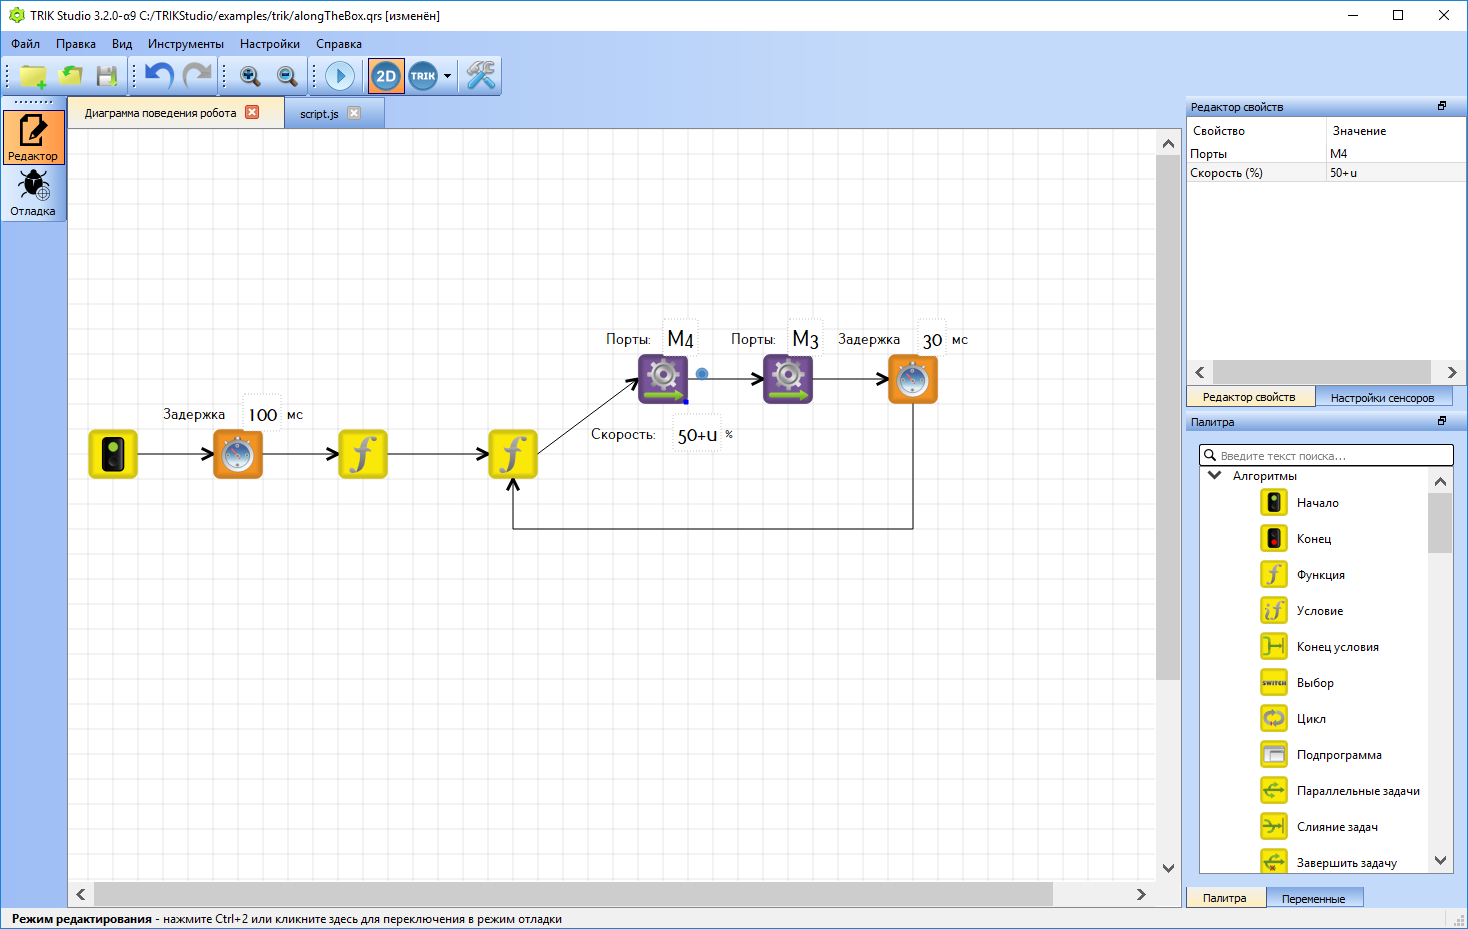
\includegraphics[width=0.9\textwidth]{trikStudio.png}}

				\footnotesize{\center{\url{https://github.com/qreal/qreal}}}
			\end{column}
			\begin{column}{0.5\textwidth}
				\center{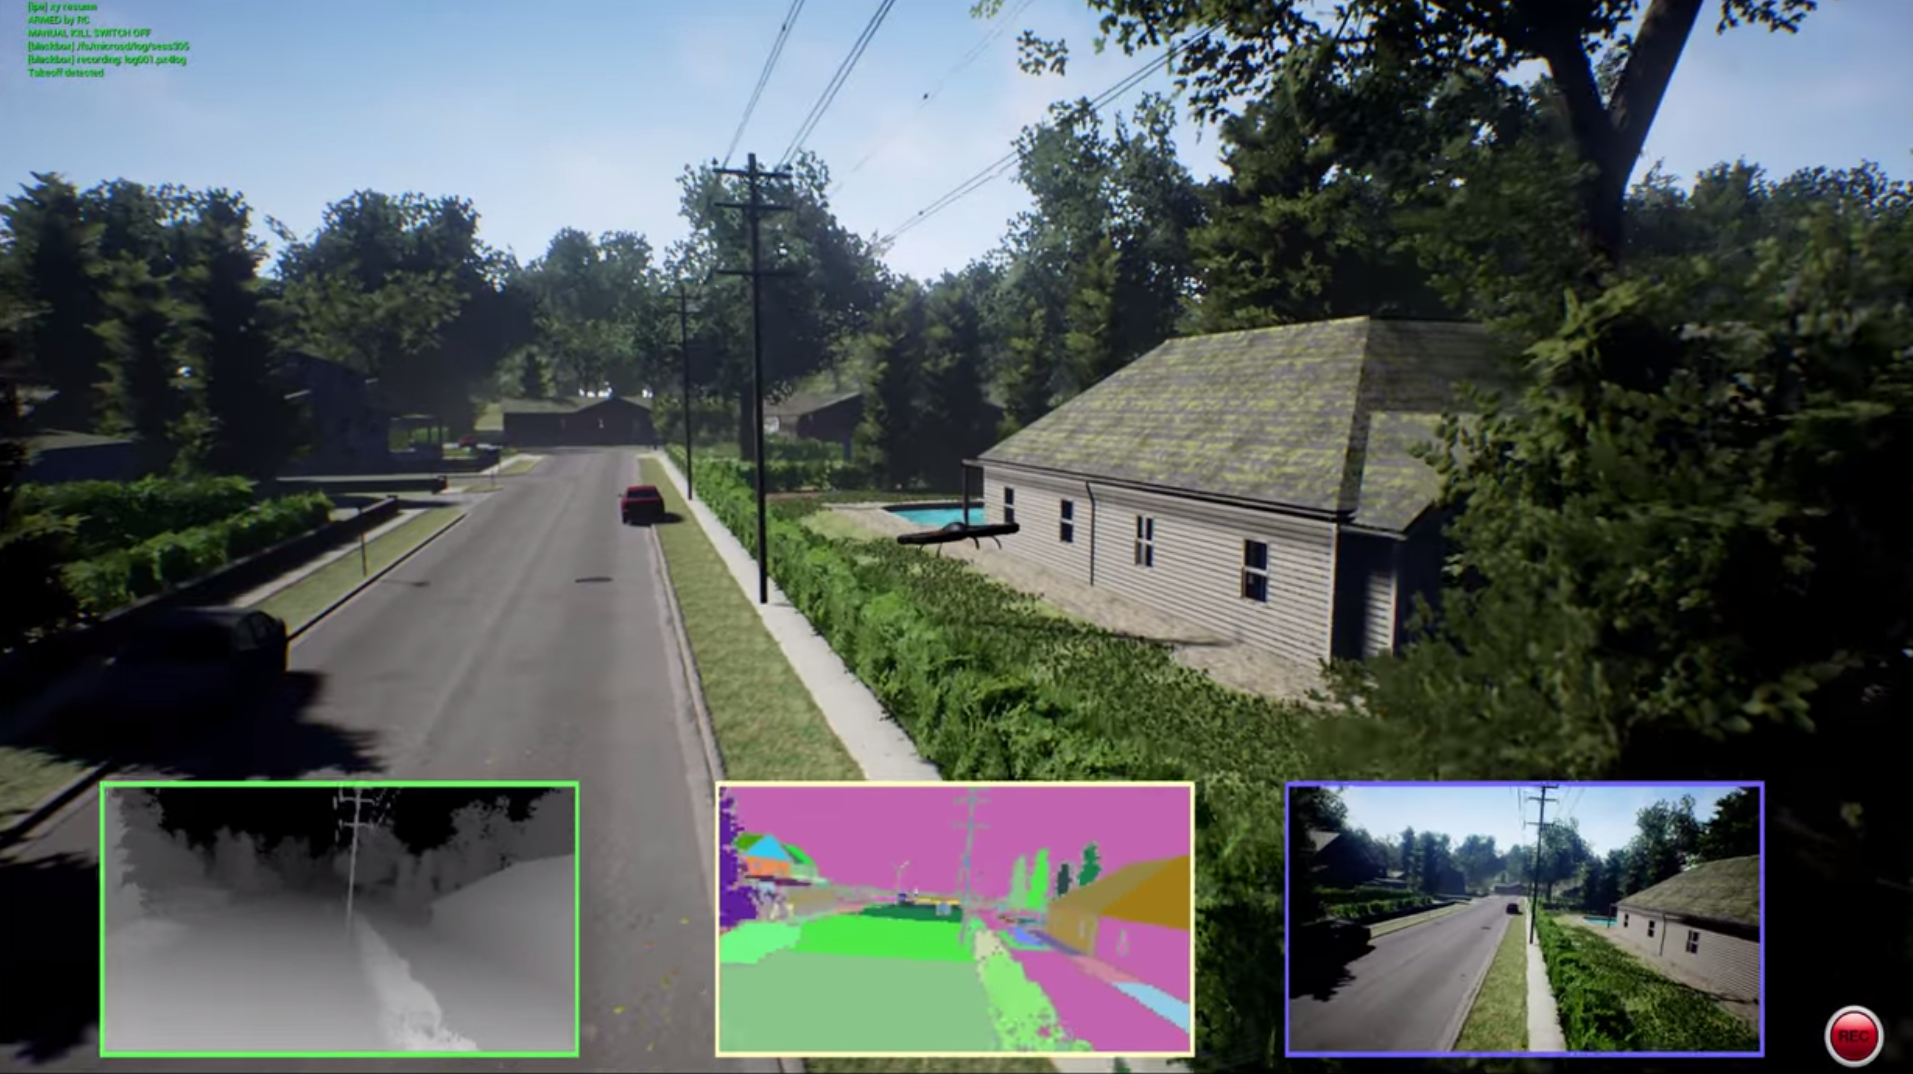
\includegraphics[width=0.98\textwidth]{airSim.png}}

				\footnotesize{\center{\url{https://github.com/microsoft/airsim}}}
			\end{column}
		\end{columns}
		\vspace{0.7cm}
		Технологии: C++, Qt

		Контакты: \texttt{yurii.litvinov@gmail.com}
	\end{frame}

\end{document}

